% !TEX TS-program = pdflatex
% !TEX encoding = UTF-8 Unicode

\documentclass[10pt, a4paper]{article}

% Essential packages
\usepackage[utf8]{inputenc}
\usepackage[T1]{fontenc}
\usepackage{helvet}
\usepackage{amssymb}
\usepackage{graphicx}
\renewcommand{\familydefault}{\sfdefault}

% Page geometry for landscape layout
\usepackage{geometry}
\geometry{a4paper, landscape, margin=1cm, top=1cm, bottom=1.5cm}

% Colors for box styling
\usepackage{xcolor}
\definecolor{boxheaderbg}{HTML}{000000}
\definecolor{boxheaderfg}{HTML}{FFFFFF}
\definecolor{boxcontentbg}{HTML}{F0F0F0}
\definecolor{boxborder}{HTML}{000000}

% tcolorbox for fixed-size boxes
\usepackage[many]{tcolorbox}

% hyperref for form fields
\usepackage{hyperref}

% Headers and footers
\usepackage{fancyhdr}
\pagestyle{fancy}
\fancyhf{}
\fancyfoot[R]{\footnotesize "Fail Forward character sheet" by Visa Lampi is licensed under CC BY-NC 4.0.}
\renewcommand{\headrulewidth}{0pt}
\renewcommand{\footrulewidth}{0pt}

% Tabularx for table formatting
\usepackage{tabularx}

\begin{document}

% Start of the form
\begin{Form}

% Two-column layout with minipages
\begin{minipage}[t]{0.48\textwidth}
    % Character box
    \begin{tcolorbox}[
        width=12.5cm,
        height=3.8cm,
        title=CHARACTER,
        colback=boxcontentbg,
        colframe=boxborder,
        coltitle=boxheaderfg,
        colbacktitle=boxheaderbg,
        fonttitle=\bfseries\sffamily\small,
        clip upper
    ]
        \begin{minipage}[c][3.3cm][c]{0.23\linewidth}
            \centering
            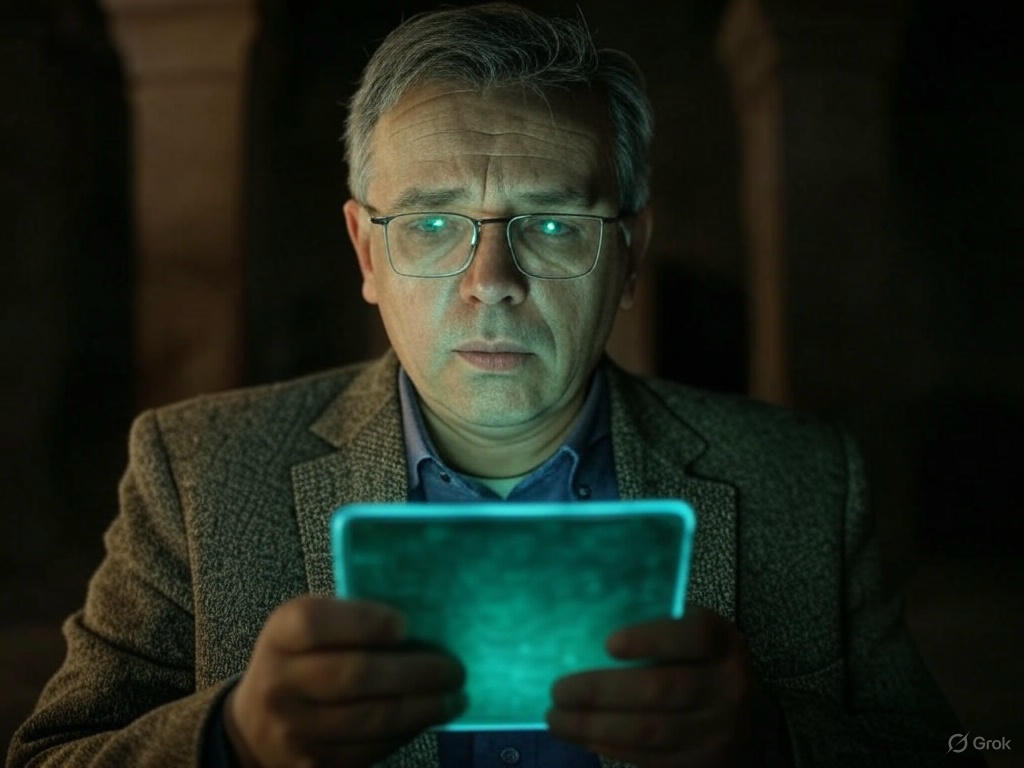
\includegraphics[width=\linewidth, height=3.3cm, keepaspectratio=true]{varn_picture.jpg}
            \vspace{0pt}
        \end{minipage}%
        \begin{minipage}[c][3.3cm][c]{0.75\linewidth}
            \centering
            \TextField[name=character_name, width=10cm, height=1cm, multiline=true]{}
        \end{minipage}
    \end{tcolorbox}

    \vspace{5mm}

    % Abilities box
    \begin{tcolorbox}[
        width=12.5cm,
        height=3cm,
        title=ABILITIES (choose 3),
        colback=boxcontentbg,
        colframe=boxborder,
        coltitle=boxheaderfg,
        colbacktitle=boxheaderbg,
        fonttitle=\bfseries\sffamily\small,
        clip upper
    ]
        \TextField[name=abilities, width=12cm, height=2.5cm, multiline=true, default={
Ancient Technology Expertise \newline
Social Media Savvy \newline
Pyramid Exploration \newline
Electrical Engineering \newline
Persuasive Communication \newline
Stealth and Infiltration \newline
Combat Proficiency \newline
Historical Knowledge \newline
Energy Field Manipulation \newline
Cryptography
        }]{}
    \end{tcolorbox}

    \vspace{5mm}

    % Background box
    \begin{tcolorbox}[
        width=12.5cm,
        height=5.5cm,
        title=BACKGROUND,
        colback=boxcontentbg,
        colframe=boxborder,
        coltitle=boxheaderfg,
        colbacktitle=boxheaderbg,
        fonttitle=\bfseries\sffamily\small,
        clip upper
    ]
        \TextField[name=background, width=12cm, height=5cm, multiline=true]{}
    \end{tcolorbox}
\end{minipage}
\hfill
\begin{minipage}[t]{0.48\textwidth}
    % Sanity box
    \begin{tcolorbox}[
        width=12.5cm,
        height=2.5cm,
        title=SANITY,
        colback=boxcontentbg,
        colframe=boxborder,
        coltitle=boxheaderfg,
        colbacktitle=boxheaderbg,
        fonttitle=\bfseries\sffamily\small,
        clip upper
    ]
        \large \hspace*{2mm}
        $\bigcirc$ \hspace{1em}
        $\bigcirc$ \hspace{1em}
        $\bigcirc$ \hspace{1em}
        $\bigcirc$ \hspace{1em}
        $\bigcirc$ \hspace{1em}
        $\bigcirc$ \\
        \textit{\footnotesize \hspace*{2mm} (6 = Sanity breaks)} \\
        \vspace{2mm}
        \textit{\footnotesize \hspace*{2mm} Check one circle each time sanity decreases.}
    \end{tcolorbox}

    \vspace{2mm}

    % Personality box
    \begin{tcolorbox}[
        width=12.5cm,
        height=3cm,
        title=PERSONALITY (choose 2),
        colback=boxcontentbg,
        colframe=boxborder,
        coltitle=boxheaderfg,
        colbacktitle=boxheaderbg,
        fonttitle=\bfseries\sffamily\small,
        clip upper
    ]
        \TextField[name=personality, width=12cm, height=2.5cm, multiline=true, default={
Adventurous \newline
Analytical \newline
Charismatic \newline
Cautious \newline
Determined \newline
Empathetic \newline
Resourceful \newline
Skeptical
        }]{}
    \end{tcolorbox}

    \vspace{2mm}

    % Handicaps box
    \begin{tcolorbox}[
        width=12.5cm,
        height=3cm,
        title=HANDICAPS (choose 2),
        colback=boxcontentbg,
        colframe=boxborder,
        coltitle=boxheaderfg,
        colbacktitle=boxheaderbg,
        fonttitle=\bfseries\sffamily\small,
        clip upper
    ]
        \TextField[name=handicaps, width=12cm, height=2.5cm, multiline=true, default={
Fear of Enclosed Spaces \newline
Allergy to Dust \newline
Technophobia \newline
Poor Night Vision \newline
Superstitious Beliefs \newline
Physical Weakness \newline
Impulsiveness \newline
Overconfidence
        }]{}
    \end{tcolorbox}

    \vspace{2mm}

    % Equipment box
    \begin{tcolorbox}[
        width=12.5cm,
        height=4.2cm,
        title=EQUIPMENT (choose 4),
        colback=boxcontentbg,
        colframe=boxborder,
        coltitle=boxheaderfg,
        colbacktitle=boxheaderbg,
        fonttitle=\bfseries\sffamily\small,
        clip upper
    ]
        \TextField[name=equipment, width=12cm, height=3.7cm, multiline=true, default={
Portable Power Generator \newline
Satellite Communication Device \newline
EMF Detector \newline
Night Vision Goggles \newline
Archaeological Digging Tools \newline
Smartphone with Social Media Apps \newline
Smoke Grenades \newline
First Aid Kit \newline
Flashlight \newline
Rope and Climbing Gear \newline
Lockpicking Set \newline
Binoculars
        }]{}
    \end{tcolorbox}
\end{minipage}

% End of the form
\end{Form}

\end{document}